% Hinh: paper/paper1/figs_revision/fig12. Caption viet lai cho QMI.
\begin{figure}[t]
  \centering
  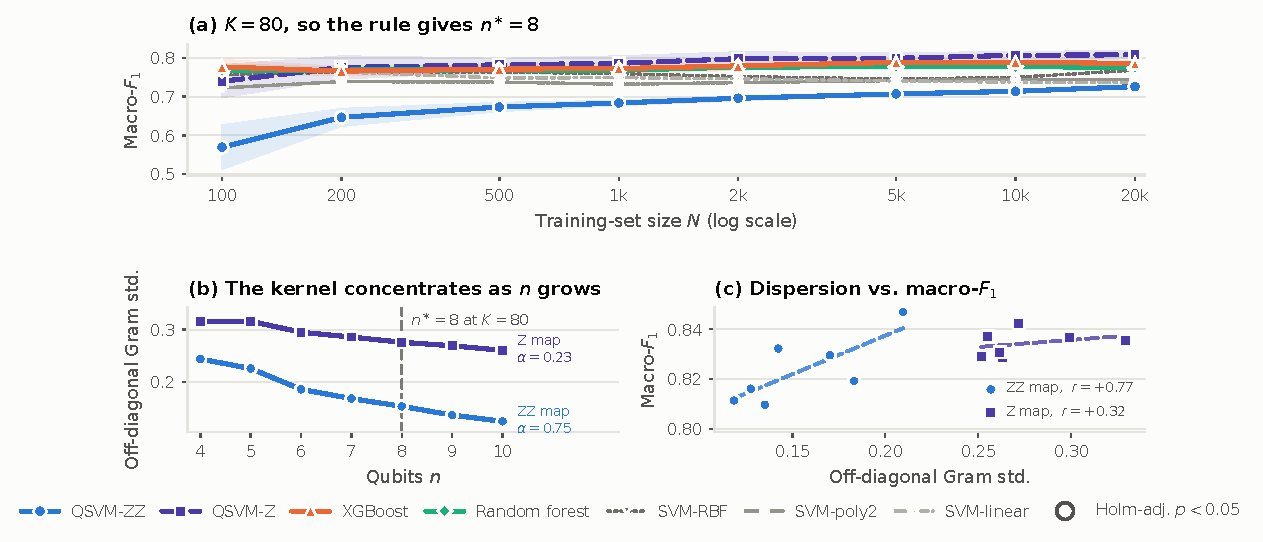
\includegraphics[width=\textwidth]{figs_revision/fig12_width_concentration.pdf}
  \caption{Circuit width. (a) The training-set-size sweep repeated at $K=80$, where the rule
    returns $n^{\ast}=8$; all $48$ paired comparisons favour the classical baseline. (b)
    Standard deviation of the off-diagonal Gram entries against width at $K=80$, with fitted
    $n^{-\alpha}$ curves ($\alpha=0.75$ for \ZZ{}, $0.23$ for \Zmap{}). (c) Off-diagonal
    dispersion against macro-$F_1$ across seven widths: $r=+0.77$ $[+0.04,+0.96]$ for \ZZ{} and
    $r=+0.32$ $[-0.57,+0.87]$ for \Zmap{}.}
  \label{fig:width}
\end{figure}
